\documentclass[aspectratio=169]{beamer}
\mode<presentation>{
	\usetheme{gemini}
    \usecolortheme{beaver}
	\useoutertheme{infolines}
	\useinnertheme{default}
}

\usepackage{appendixnumberbeamer}
\usepackage{tikz}
\usepackage{minted}

\usemintedstyle{lovelace}
\setminted{autogobble=true}

% Notes Options
% \setbeameroption{hide notes}
% \setbeameroption{show notes}
% \setbeameroption{show only notes}

% Preamble Content
\title[MetPy Cross Sections (288)]{Cross Section Analysis in MetPy}
\author[Thielen et al.]{Jonathan E. Thielen, R. M. May, and J. R. Leeman}
\date[January 7, 2019]{Ninth Symposium on Advances in Modeling and Analysis Using Python\\ \ \\January 7, 2019}
\subject{Ninth Symposium on Advances in Modeling and Analysis Using Python}


%\AtBeginSection[]{
%	\begin{frame}
%		\frametitle{Outline}
%		\tableofcontents[currentsection]
%	\end{frame}
%}

%%%%%%%%%%%%%%%%%%
%% The Document %%
%%%%%%%%%%%%%%%%%%
\begin{document}

% Title
\frame{\titlepage}

\begin{frame}
	\frametitle{Vertical Cross Sections}
    Often used in analysis of:
    \begin{itemize}
      \item Convective systems
      \item Isentropic ascent
      \item Tropopause folds
      \item Conditional Symmetric Instability (CSI)
    \end{itemize}
    
    \ 
    
    \begin{center}
        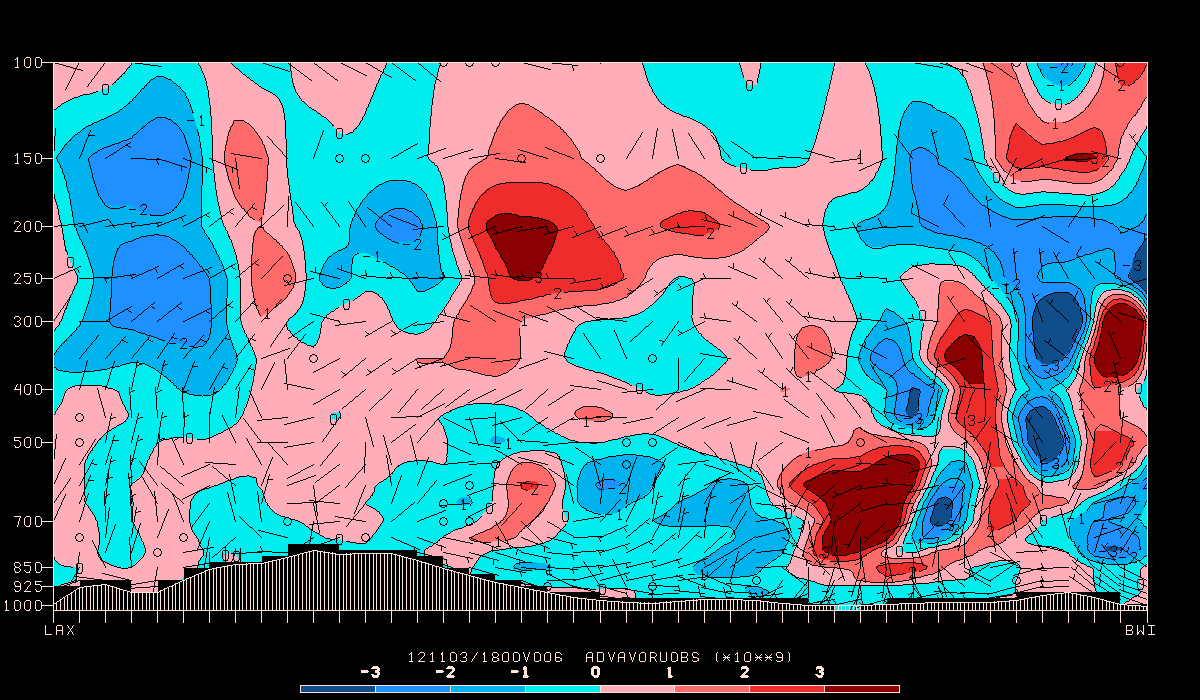
\includegraphics[height=1.5in]{figures/gempak_cross.png}
    \end{center}
\end{frame}

\begin{frame}
    \frametitle{Examples from MetPy}
    \begin{center}
        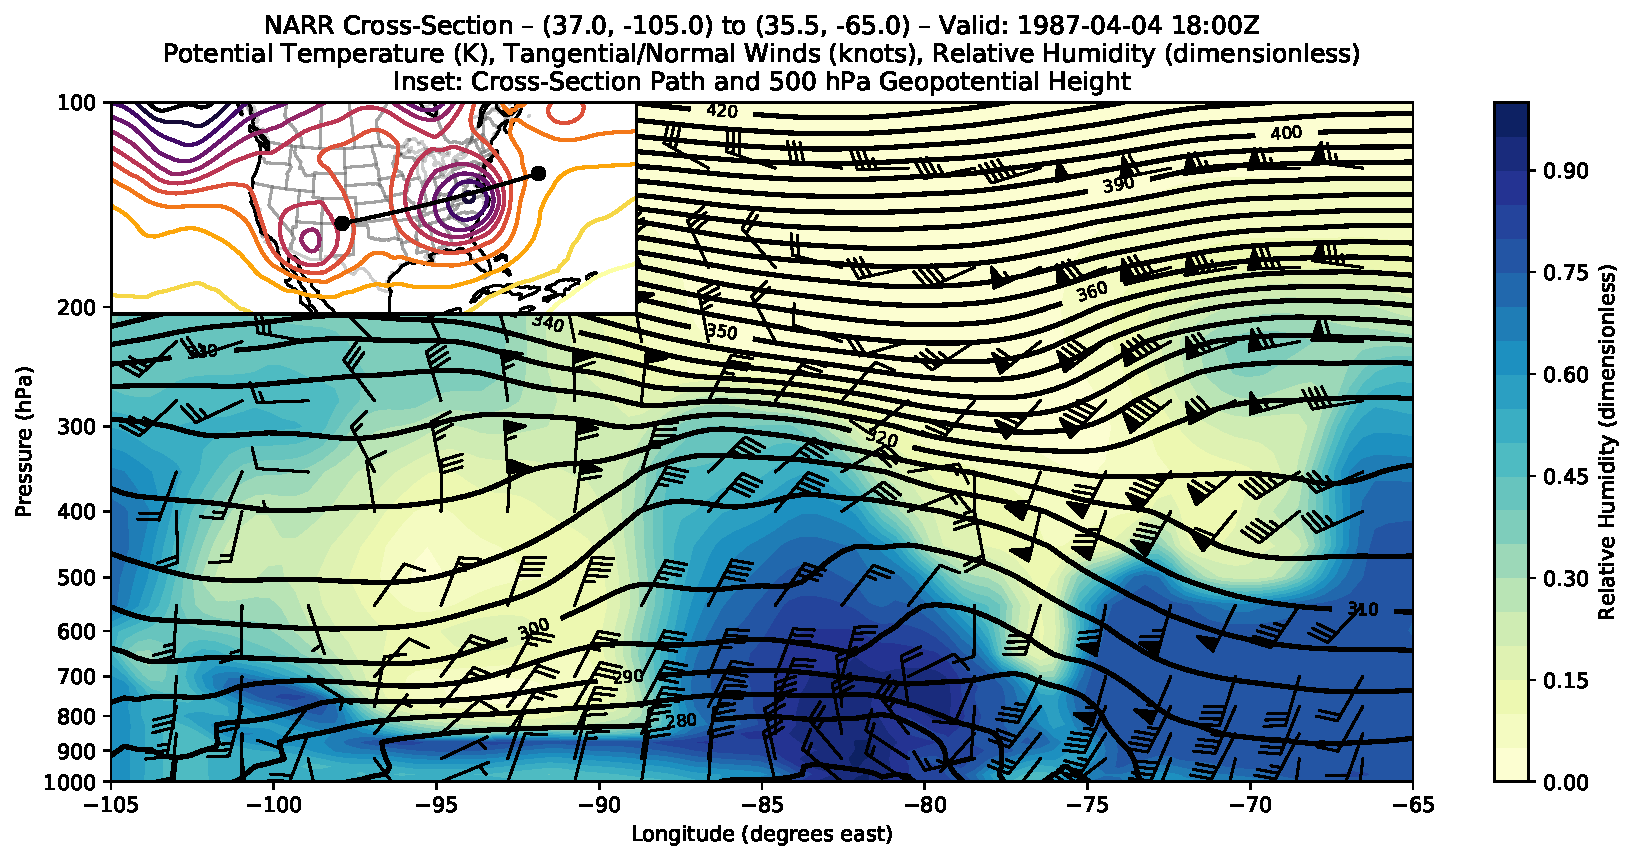
\includegraphics[height=2.5in]{figures/basic_example_narr.pdf}
    \end{center}
\end{frame}

\begin{frame}
    \frametitle{Examples from MetPy}
    \begin{center}
        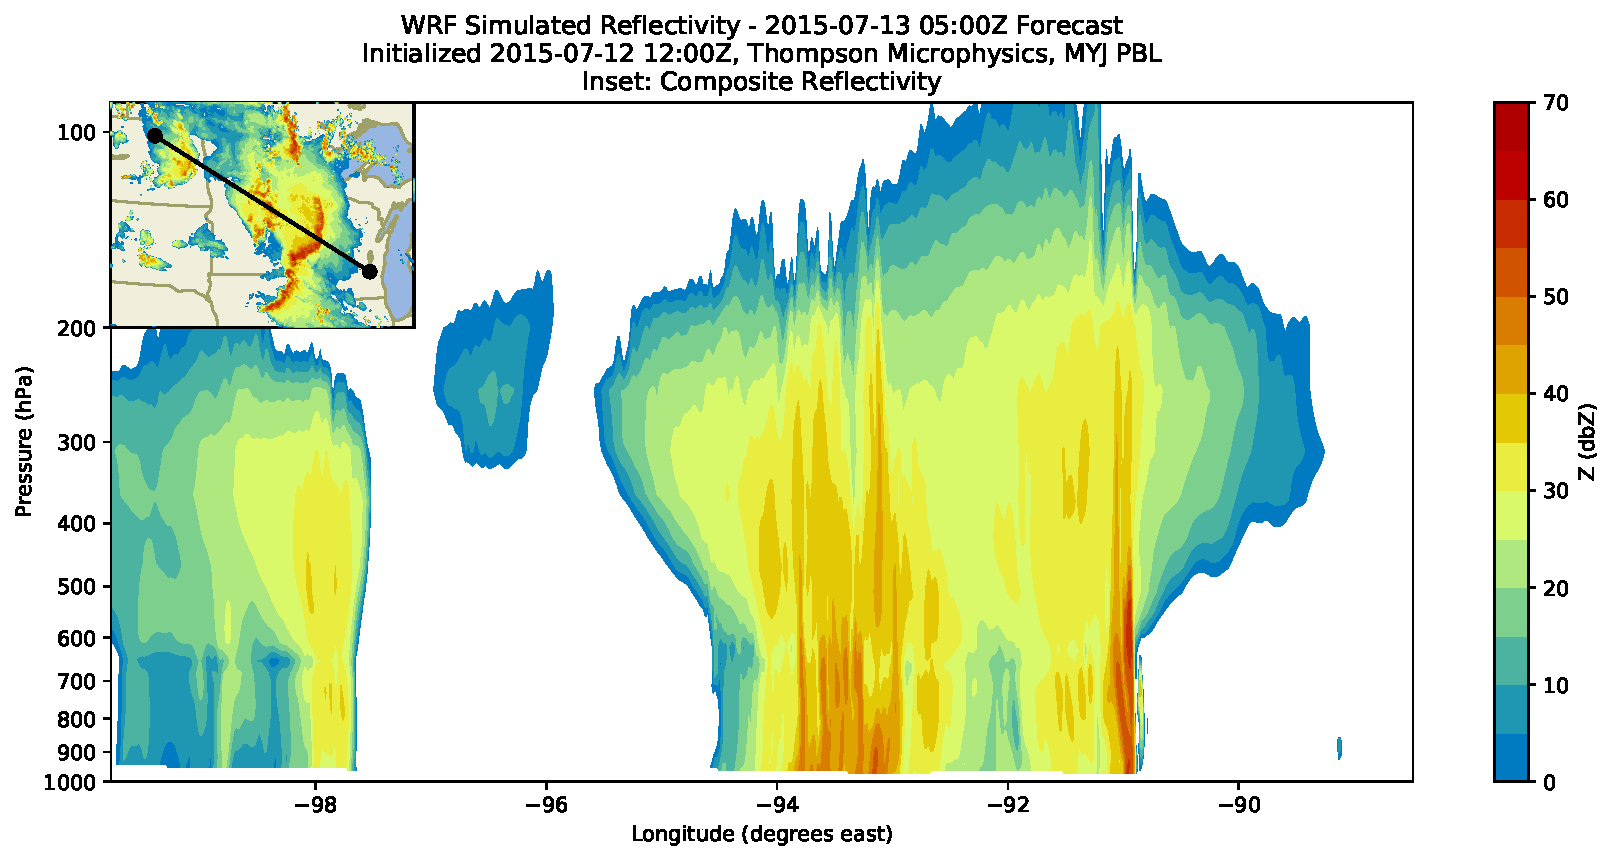
\includegraphics[height=2.5in]{figures/wrf_refl.pdf}
    \end{center}
\end{frame}

\begin{frame}
    \frametitle{Examples from MetPy}
    \begin{center}
        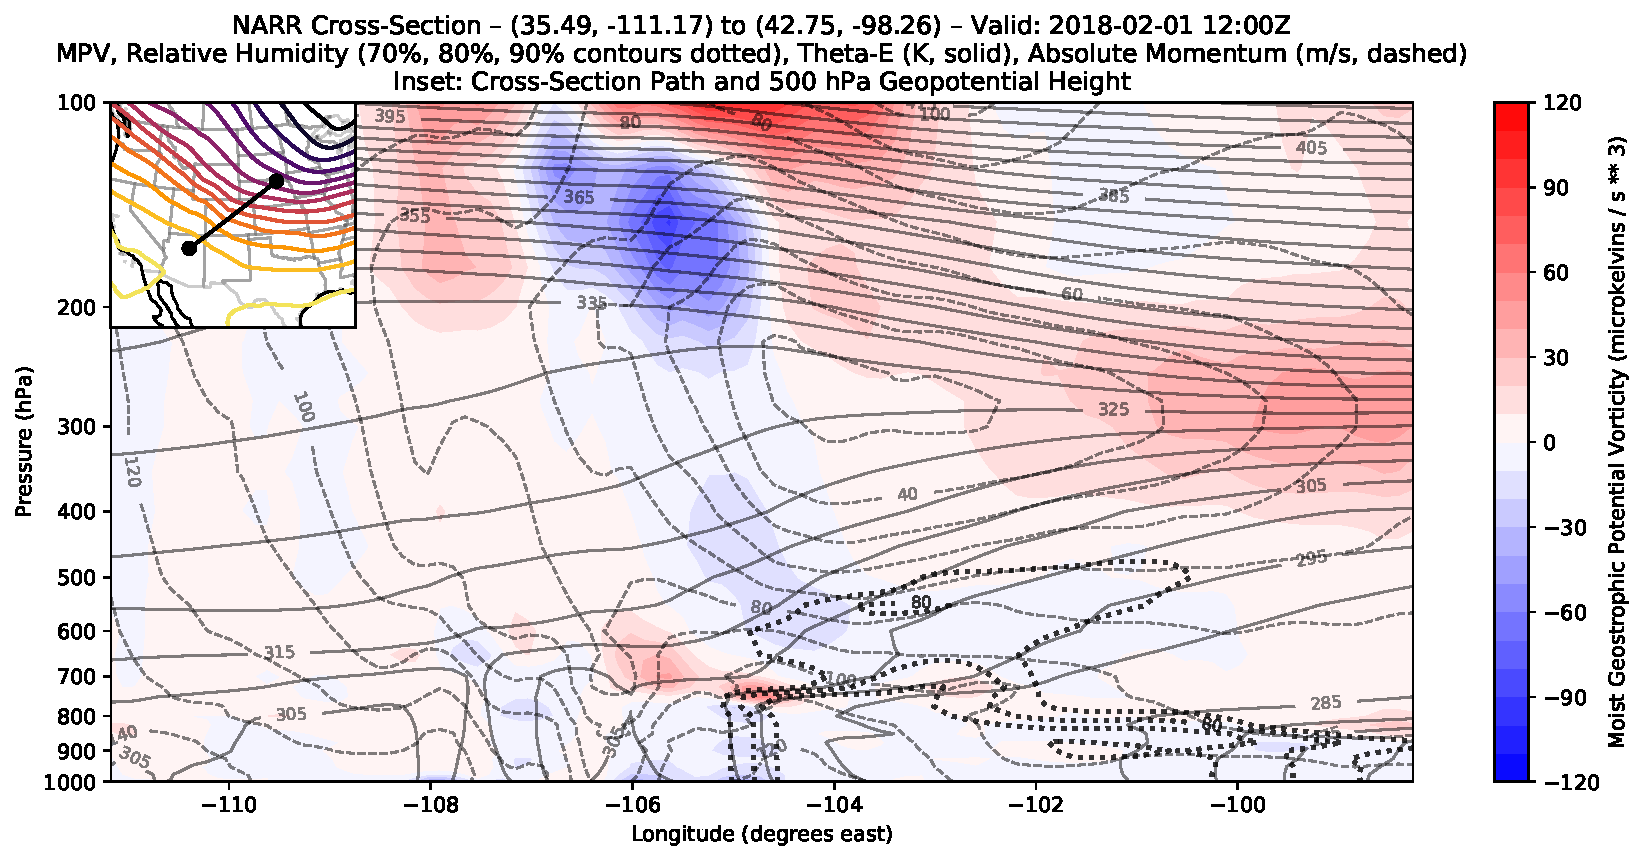
\includegraphics[height=2.5in]{figures/csi_example_narr.pdf}
    \end{center}
\end{frame}

\begin{frame}
    \frametitle{How It Works}
    Stop by the poster (288) to find out more...
\end{frame}

\begin{frame}[fragile]
    \frametitle{How It Works}
    ...but the short answer is xarray.
    
    \ 
    
    \begin{minted}{python}
      import xarray as xr
      from metpy.interpolate import cross_section

      # Parse for CRS and coordinate types
      data = xr.open_dataset('data.nc').metpy.parse_cf()

      # Interpolate to cross-sectional slice
      cross = cross_section(data, (37.0, -105.0), (35.5, -65.0))
    \end{minted}
\end{frame}

\end{document}